\chapter{Pertemuan 2}

\section{Issues \#11}
Pada \textit{issues \#11} (\textit{Cek mainActivity}) \textit{mainActivity} Merupakan activity yang utama ketika program dijalankan. Pada saat cek mainActivity, Program sudah bisa berjalan tanpa error. 
\begin{figure}[]
        \centering
        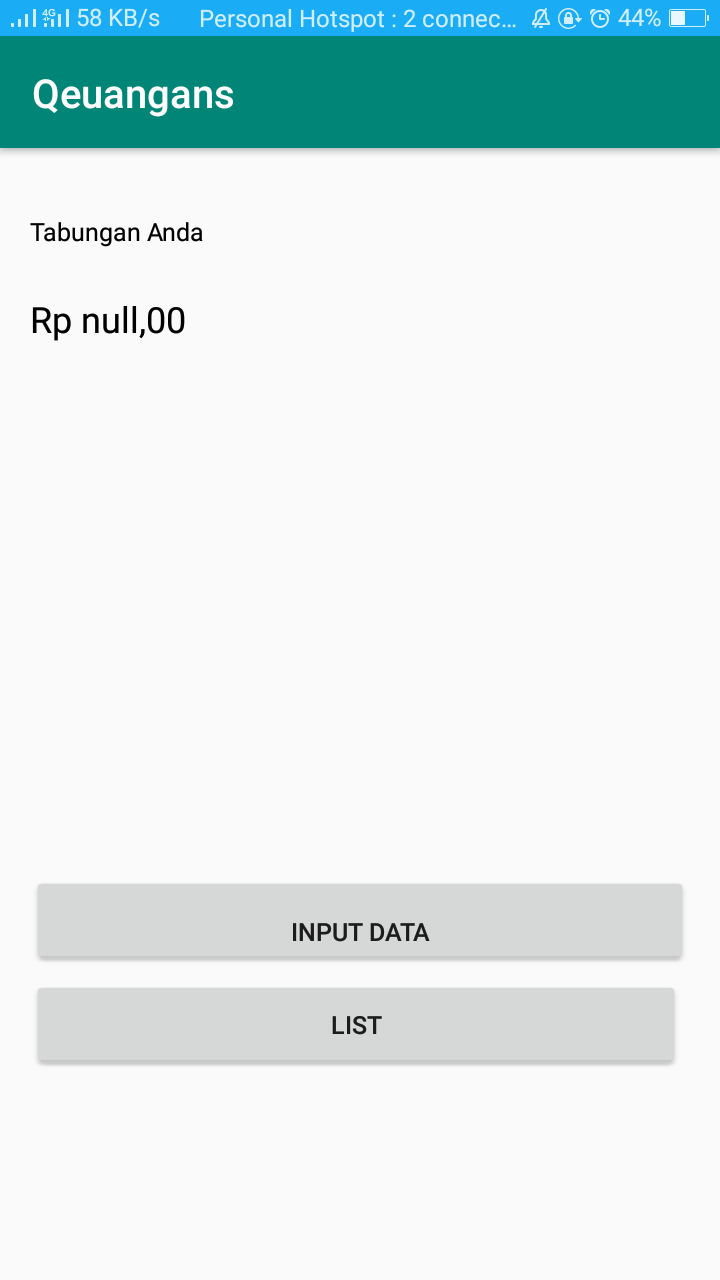
\includegraphics[scale = 0.3]{pictures/mainActivity.png}
        \caption{Gambar tampilan mainActivity}
        \label{mainActivity}
\end{figure}

\section{Issues \#12}
Pada \textit{issues \#12} (Penambahan Fitur Laporan) merupakan penambahan laporan.java pada aplikasi, penambahan fitur laporan ini menggunakan arraylist
\begin{verbatim}

        import androidx.appcompat.app.AppCompatActivity;

        import android.database.Cursor;
        import android.os.Bundle;
        import android.widget.ArrayAdapter;
        import android.widget.ListView;
        import android.widget.Toast;
        
        import java.util.ArrayList;
        
        public class laporan extends AppCompatActivity {
        
            DatabaseHelper db;
            ListView listLaporanK;
        
            @Override
            protected void onCreate(Bundle savedInstanceState) {
                super.onCreate(savedInstanceState);
                setContentView(R.layout.activity_laporan);
        
                listLaporanK = findViewById(R.id.listLaporanK);
        
                LK = new ArrayList<>();
        
                db = new DatabaseHelper(this);
        
                datalaporankeluar();
            }
        
            private void datalaporankeluar() {
                Cursor cursor = db.datalaporankeluar();
                if (cursor.getCount() == 0) {
                    Toast.makeText(this, "TIDAK ADA DATA", Toast.LENGTH_SHORT).show();
                } else {
                    while (cursor.moveToNext()) {
                        LK.add("\n" + cursor.getString(0) + "\n" + "Tanggal : " + cursor.getString(5) + "\n" + "\n" + "Pemasukan : " + cursor.getString(1)
                                + "\n" + "Jumlah : Rp " + cursor.getString(2) + ",00" + "\n" + "\n" + "Pengeluaran : " + cursor.getString(3)
                                + "\n" + "Jumlah : Rp" + cursor.getString(4) + ",00" + "\n");
                    }
                }
            }
        }
\end{verbatim}

\section{Issues \#13}
Pada \textit{issues \#13} (Tombol laporan tidak muncul pada aplikasi). Pada issues ini, tombol laporan tidak muncul pada aplikasi karena tombol tersebut belum dipanggil untuk dimunculkan. untuk memanggilnya menggunakan \begin{verbatim}
tombolLaporan = findViewById(R.id.tombolLaporan);
\end{verbatim}
disini berarti tombolLaporan ini dihubungkan dengan id dari tombol yang ada di mainActivity.XML dengan id tombolLaporan.

\section{Issues \#14}
Pada \textit{issues \#14} (\textit{Error: Undefined Method}) \textit{Undefined Method} merupakan jenis \textit{error} yang disebaban karena ketika method dipanggil tetapi method yang dipanggil tidak ada, maka akan muncul \textit{Undefined Method}. Solusi yang digunakan adalah dengan membuat method yang dipanggil.\\
Pemanggilan method:
\begin{verbatim}
Laporan();
\end{verbatim}
Method yang dipanggil:
\begin{verbatim}
public void Laporan(View view) {
    Intent intent = new Intent(MainActivity.this, laporan.class);
    startActivity(intent);
}
\end{verbatim}


\section{Issues \#15}
Pada \textit{issues \#15} (\textit{Error: ID is not Defined Anywhere}) \textit{ID is not Defined Anywhere} merupakan sebuah \textit{error}. \textit{Error} ini terjadi ketika sebuah id tombol pada activity\_main.XML ( android:id="Laporan") tidak memiliki ID yang benar, maka solusinya adalah memberikan id yang benar dengan menambahkan @+id pada awal kata "Laporan" contoh:
\begin{verbatim}
android:id="@+id/tombolLaporan"
\end{verbatim}
penggunaan @+id disini agar sesuai dengan penulisan yang digunakan pada android. 

\section{Issues \#16}
Pada \textit{issues \#16} (\textit{Error: Missing Constraints}) \textit{Missing Constraints} adalah \textit{error} yang terjadi ketika sebuah tampilan yang ada tidak ditentukan posisinya secara pasti. Contoh tampilan tanpa cnstraint pada activity\_main.XML: 
\begin{verbatim}
<TextView android:layout_width="wrap_content"
android:layout_height="wrap_content"
android:layout_alignParentTop="true"
android:layout_marginTop="18dp"
android:textColor="#000000"
android:text="@string/Tabungan_anda" 
\end{verbatim}
Jika posisi tidak ditentukan, maka yang terjadi adalah, tampilan tersebut akan otomatis berada pada (0,0) bagian layar atau di posisi kiri atas ketika aplikasi dijalankan. Solusi error tersebut adalah dengan menentukan posisinya. 
\begin{verbatim}
<TextView android:layout_width="wrap_content"
android:layout_height="wrap_content"
android:layout_alignParentTop="true"
android:layout_marginTop="18dp"
android:textColor="#000000"
android:text="@string/Tabungan_anda"
app:layout_constraintTop_toBottomOf="@+id/TombolLaporankeluar"
\end{verbatim}
layout\_constraintTop\_toBottomOf merupakan penentuan posisi pada bagian bawah yang dihubungkan dengan tampilan yang memiliki id "TombolLaporankeluar" yang ada pada activity\_main.XML.


\section{Issues \#17}
Pada \textit{issues \#17} (\textit{Error: Cannot Resolve Method add(java.lang.string)}) \textit{Cannot Resolve Method add(java.lang.string} adalah ketika method tidak bisa menambahkan value string pada arraylist yang akan ditampilkan. 

\section{Issues \#18}
Pada \textit{issues \#18} (Mengkoneksikan Database) Untuk mengkoneksikan database dapat menggunakan perintah:
\begin{verbatim}
db = new DatabaseHelper(this); 
\end{verbatim}
Perintah ini dimasukan pada file MainActivity.java

\section{Issues \#19}
Pada \textit{issues \#19} (\textit{Error: Cannot return value from void method.}) \textit{Error: Cannot return value from void method} merupakan sebuah \textit{error} yang disebabkan karena mencoba menggunakan perintah return(mengembalikan nilai) pada method void. Contoh pada DatabaseHelper.java:
\begin{verbatim}
public void datalaporankeluar(){ 
        SQLiteDatabase db = this.getReadableDatabase();
        Cursor saldo;
        saldo = db.rawQuery("SELECT SUM(" +COL3+")-SUM(" +COL5+") FROM "+TBLNAME, null);
        return saldo;
    }
\end{verbatim}
Sedangkan void sendiri merukpakan method yang tidak mengembalikan nilai sehingga return tidak bisa digunakan pada method void. Untuk solusinya yaitu dengan membuat methud tersebut menjadi function. Contoh: 
\begin{verbatim}
public Cursor datalaporankeluar(){ // Cannot return value from void method.  // Solusi ERROR 18. Issues #20 //
    SQLiteDatabase db = this.getReadableDatabase();
    Cursor saldo;
    saldo = db.rawQuery("SELECT SUM(" +COL3+")-SUM(" +COL5+") FROM "+TBLNAME, null);
    return saldo;
}
\end{verbatim}
Void disini diubah menjadi "cursor" karena digunakan untuk menganmbil value suatu data pada database yang di eksekusi dengan perintah "return saldo;"

\section{Issues \#20}
Pada \textit{issues \#20} (Koneksi ke Database) Untuk membuat koneksi ke database mengunakan perintah:
\begin{verbatim}
db = new DatabaseHelper(this);
\end{verbatim}